\documentclass[12pt, openright, oneside, a4paper, english, brazilian]{abntex2}


% ---
% Pacotes
% ---
\usepackage{lmodern}			% Usa a fonte Latin Modern			
\usepackage[T1]{fontenc}		% Selecao de codigos de fonte.
\usepackage[utf8]{inputenc}		% Codificacao do documento (conversão automática dos acentos)
\usepackage{indentfirst}		% Indenta o primeiro parágrafo de cada seção.
\usepackage{color}				% Controle das cores
\usepackage{graphicx}			% Inclusão de gráficos
\usepackage{microtype} 			% para melhorias de justificação
\usepackage[brazilian,hyperpageref]{backref}	 % Paginas com as citações na bibl
\usepackage[alf]{abntex2cite}	% Citações padrão ABNT
\usepackage{lipsum}     %Gerador de texto aleatorio em Latim

\usepackage[normalem]{ulem} %sublinhar linhas e permitir quebrar linhas
\usepackage{amssymb} %necessário para $\square$
\usepackage{amsmath}
\usepackage{booktabs}
\usepackage{array}


% --- 
% CONFIGURAÇÕES DE PACOTES
% --- 

% ---
% Configurações do pacote backref
% Usado sem a opção hyperpageref de backref
\renewcommand{\backrefpagesname}{Citado na(s) página(s):~}
% Texto padrão antes do número das páginas
\renewcommand{\backref}{}
% Define os textos da citação
\renewcommand*{\backrefalt}[4]{
	\ifcase #1 %
		Nenhuma citação no texto.%
	\or
		Citado na página #2.%
	\else
		Citado #1 vezes nas páginas #2.%
	\fi}%
% ---


\usepackage{enumitem}
\usepackage{tikz}
\usepackage{listings}
\usetikzlibrary{positioning, arrows.meta, shapes.geometric}

% ----------------------------------
% --- Configurações da capa do IFPR
% ----------------------------------
\renewcommand{\imprimircapa}{%
    \begin{capa}%
        \center
        \begin{figure*}
            \centering
            
\includegraphics[height=2.5cm]{figuras/logo-ifpr.png}
        \end{figure*}
        \vspace*{\fill}
        {\ABNTEXchapterfont\large\imprimirautor}\\
        \vspace*{\fill}
        \vspace{2.5cm}{\ABNTEXchapterfont\bfseries\LARGE\imprimirtitulo}\\
        \vspace*{\fill}
        \vspace*{\fill}
        \vspace{2.5cm}
        {\large\imprimirlocal}\\
        \par
        {\large\imprimirdata}\\
        \vspace*{1cm}
    \end{capa}
}


% ---
% Informações de dados para CAPA e FOLHA DE ROSTO
% ---
\titulo{PROPOSTA DE DESENVOLVIMENTO DE ATIVIDADES DE EXTENSÃO: Bracelete Inteligente com ESP32 para Auxílio a Pessoas com Baixa Visão}    %Título

\autor{Matheus Vitor Lourenço Schionato\\Vairtles Nehisen Mounkassa Liel}  %Autores
\local{Pinhais}
\data{2026}
% \orientador{Prof. Fulano de Tal}
% \coorientador{Prof. Deltrano de Tal}
\instituicao{%
  Instituto Federal do Paraná -- IFPR
  \par
  Campus Pinhais
  \par
  Bacharelado em Ciência da Computação}
\tipotrabalho{Proposta de Desenvolvimento de Atividades de Extensão}       % Tipo de trabalho

% O preambulo deve conter o tipo do trabalho, o objetivo, o nome da instituição e a área de concentração. Preambulo aparece na folha de Rosto
\preambulo{Proposta de atividades extensionistas apresentada à disciplina de Práticas de Extensão V, do curso de Bacharelado em Ciência da Computação do Instituto Federal do Paraná, Campus Pinhais, sob a orientação do professor responsável.}
% ---


% ---
% Configurações de aparência do PDF final

% alterando o aspecto da cor azul
\definecolor{black}{RGB}{0,0,0}




% informações do PDF
\makeatletter
\hypersetup{
     	%pagebackref=true,
		pdftitle={\@title}, 
		pdfauthor={\@author},
    	pdfsubject={\imprimirpreambulo},
	    pdfcreator={LaTeX with abnTeX2},
		pdfkeywords={abnt}{latex}{abntex}{abntex2}{trabalho acadêmico}, 
		colorlinks=true,       		% false: boxed links; true: colored links
    	linkcolor=black,          	% color of internal links
    	citecolor=black,        		% color of links to bibliography
    	filecolor=magenta,      		% color of file links
		urlcolor=black,
		bookmarksdepth=4
}
\makeatother
% --- 

% ---
% Posiciona figuras e tabelas no topo da página quando adicionadas sozinhas
% em um página em branco. Ver https://github.com/abntex/abntex2/issues/170
\makeatletter
\setlength{\@fptop}{5pt} % Set distance from top of page to first float
\makeatother
% ---

% ---
% Possibilita criação de Quadros e Lista de quadros.
% Ver https://github.com/abntex/abntex2/issues/176
%
\newcommand{\quadroname}{Quadro}
\newcommand{\listofquadrosname}{Lista de quadros}

\newfloat[chapter]{quadro}{loq}{\quadroname}
\newlistof{listofquadros}{loq}{\listofquadrosname}
\newlistentry{quadro}{loq}{0}

% configurações para atender às regras da ABNT
\setfloatadjustment{quadro}{\centering}
\counterwithout{quadro}{chapter}
\renewcommand{\cftquadroname}{\quadroname\space} 
\renewcommand*{\cftquadroaftersnum}{\hfill--\hfill}

\setfloatlocations{quadro}{hbtp} % Ver https://github.com/abntex/abntex2/issues/176
% ---

% --- 
% Espaçamentos entre linhas e parágrafos 
% --- 

% O tamanho do parágrafo é dado por:
\setlength{\parindent}{1.3cm}

% Controle do espaçamento entre um parágrafo e outro:
\setlength{\parskip}{0.2cm}  % tente também \onelineskip

% ---
% compila o indice
% ---
\makeindex
% ---

% ----
% Início do documento
% ----


\titulo{RELATÓRIO PARCIAL DE ATIVIDADES DE EXTENSÃO: BRACELETE INTELIGENTE COM ESP32 PARA AUXÍLIO À ORIENTAÇÃO DE PESSOAS COM BAIXA VISÃO}
\tipotrabalho{Relatório Parcial de Atividades de Extensão}
\preambulo{Relatório parcial de atividades extensionistas apresentado à disciplina de Práticas de Extensão V, do curso de Bacharelado em Ciência da Computação do Instituto Federal do Paraná, Campus Pinhais, sob a orientação do professor responsável.}

\begin{document}

\selectlanguage{brazilian}
\frenchspacing

\imprimircapa
\imprimirfolhaderosto

\setlength{\absparsep}{18pt}
\begin{resumo}
Este relatório parcial apresenta o andamento da ação de extensão que desenvolve um protótipo de bracelete inteligente baseado em microcontrolador ESP32, voltado a auxiliar pessoas com baixa visão na orientação em ambientes internos. Durante o detalhamento do projeto físico, a configuração do bracelete foi definida sem sensor de distância, e a detecção passou a ser feita por balizas \textit{Bluetooth Low Energy} (BLE) fixadas em pontos de interesse do ambiente, como portas e mesas. O bracelete, implementado em uma placa ESP32-C3, varre continuamente os anúncios das balizas, estima a distância de cada uma pela intensidade do sinal recebido (RSSI), aciona um motor de vibração conforme a baliza mais próxima e envia a lista de pontos detectados a um \textit{smartphone} em sentido único, por notificações BLE. No celular, uma página web que usa as interfaces Web Bluetooth e de síntese de voz apresenta os pontos em alto contraste e os anuncia em áudio, sem necessidade de instalar aplicativo. Até o momento foram concluídos o firmware do bracelete e da baliza, a interface web, um modo de demonstração e testes funcionais de comunicação. Os testes confirmaram a transmissão ESP32 $\rightarrow$ celular e a detecção simultânea de mais de uma baliza, mas mostraram que a estimativa de distância em metros pelo RSSI é instável com as placas utilizadas: com as placas a cerca de 1~m, a interface chegou a indicar 20~m. Como próxima etapa, a distância em metros será substituída por zonas de proximidade calibradas experimentalmente, seguidas da montagem física do bracelete e da validação com o público-alvo.

\textbf{Palavras-chave}: Tecnologia assistiva; ESP32; Bluetooth Low Energy; Baixa visão; Sistemas embarcados.
\end{resumo}

\begin{resumo}[Abstract]
\begin{otherlanguage*}{english}
This partial report presents the progress of an extension project that develops a smart wristband prototype based on the ESP32 microcontroller, intended to help people with low vision orient themselves indoors. While detailing the physical design, the wristband was defined without a distance sensor, so detection now relies on Bluetooth Low Energy (BLE) beacons placed at points of interest such as doors and tables. The wristband, built on an ESP32-C3 board, continuously scans beacon advertisements, estimates the distance to each one from the received signal strength (RSSI), drives a vibration motor according to the nearest beacon and sends the list of detected points to a smartphone in a single direction through BLE notifications. On the phone, a web page using the Web Bluetooth and speech synthesis interfaces shows the points in high contrast and announces them by voice, with no app installation. So far, the wristband and beacon firmware, the web interface, a demonstration mode and functional communication tests have been completed. The tests confirmed ESP32-to-phone transmission and simultaneous detection of more than one beacon, but showed that RSSI-based distance in meters is unstable with the boards used: with the boards about 1~m apart, the interface reported up to 20~m. As next steps, distance in meters will be replaced by experimentally calibrated proximity zones, followed by the physical assembly of the wristband and validation with the target audience.

\vspace{\onelineskip}
\noindent
\textbf{Keywords}: Assistive technology; ESP32; Bluetooth Low Energy; Low vision; Embedded systems.
\end{otherlanguage*}
\end{resumo}

\pdfbookmark[0]{\listfigurename}{lof}
\listoffigures*
\cleardoublepage

\pdfbookmark[0]{\listofquadrosname}{loq}
\listofquadros*
\cleardoublepage

\pdfbookmark[0]{\listtablename}{lot}
\listoftables*
\cleardoublepage

\begin{siglas}
  \item[API] Interface de Programação de Aplicações (\textit{Application Programming Interface})
  \item[BLE] Bluetooth de Baixo Consumo (\textit{Bluetooth Low Energy})
  \item[CDC] Classe de Dispositivo de Comunicação USB (\textit{Communications Device Class})
  \item[GATT] Perfil de Atributos Genérico (\textit{Generic Attribute Profile})
  \item[GPIO] Pinos de Entrada e Saída de Uso Geral (\textit{General Purpose Input/Output})
  \item[HTTPS] Protocolo de Transferência de Hipertexto Seguro
  \item[IFPR] Instituto Federal do Paraná
  \item[LBI] Lei Brasileira de Inclusão da Pessoa com Deficiência (Lei nº 13.146/2015)
  \item[MTU] Unidade Máxima de Transmissão (\textit{Maximum Transmission Unit})
  \item[OMS] Organização Mundial da Saúde
  \item[PWM] Modulação por Largura de Pulso (\textit{Pulse Width Modulation})
  \item[RSSI] Indicador de Intensidade do Sinal Recebido (\textit{Received Signal Strength Indicator})
  \item[TA] Tecnologia Assistiva
  \item[USB] Barramento Serial Universal (\textit{Universal Serial Bus})
  \item[UUID] Identificador Único Universal (\textit{Universally Unique Identifier})
\end{siglas}

\begin{simbolos}
  \item[$d$] Distância estimada entre o bracelete e a baliza, em metros
  \item[$A$] RSSI de referência medido a 1~m da baliza, em dBm
  \item[$n$] Expoente de perda de percurso do ambiente (adimensional)
  \item[$r_k$] Amostra de RSSI recebida no anúncio $k$, em dBm
  \item[$R_k$] RSSI suavizado após a amostra $k$, em dBm
  \item[$\alpha$] Fator de suavização da média móvel exponencial
\end{simbolos}


\pdfbookmark[0]{\contentsname}{toc}
\tableofcontents*
\cleardoublepage

\textual

\chapter{INTRODUÇÃO}
\label{cap:introducao}

A locomoção independente em ambientes internos ainda é uma dificuldade cotidiana para pessoas com baixa visão. Segundo a \citeonline{oms2019vision}, pelo menos 2,2 bilhões de pessoas no mundo têm algum tipo de deficiência visual, e boa parte delas mantém resíduo visual que não é suficiente para identificar com segurança portas, móveis e outros pontos de referência. No Brasil, a Lei Brasileira de Inclusão \cite{brasil2015lbi} assegura o direito à acessibilidade e reconhece a tecnologia assistiva como meio de ampliar a autonomia dessas pessoas.

Este relatório parcial descreve o andamento da ação de extensão proposta na disciplina de Práticas de Extensão III e executada na disciplina de Práticas de Extensão V do curso de Bacharelado em Ciência da Computação do IFPR -- Campus Pinhais. A ação consiste no desenvolvimento de um protótipo de bracelete inteligente baseado no microcontrolador ESP32, de baixo custo e com componentes comerciais, que auxilie pessoas com baixa visão a se orientar em um ambiente.

\section{Identificação da ação extensionista}
\label{sec:identificacao}

\begin{itemize}
    \item \textbf{Público-alvo:} pessoas com baixa visão e deficiência visual que precisam de apoio para localizar pontos de referência em ambientes internos, além da comunidade técnica e escolar interessada em tecnologias assistivas abertas;
    \item \textbf{Período:} segundo semestre letivo de 2026. Este relatório cobre as atividades realizadas até o fim de setembro de 2026;
    \item \textbf{Local:} IFPR -- Campus Pinhais, com parte do desenvolvimento e dos testes realizada pelos estudantes fora do campus, com as mesmas placas e ferramentas;
    \item \textbf{Extensionistas:} Matheus Vitor Lourenço Schionato e Vairtles Nehisen Mounkassa Liel, discentes do Bacharelado em Ciência da Computação, sob orientação do professor responsável pela disciplina.
\end{itemize}

\section{Delimitação do problema}
\label{sec:delimitacao}

A proposta original previa um bracelete com sensor ultrassônico para detectar obstáculos à frente do usuário. Durante o detalhamento do projeto físico, a equipe definiu uma configuração do bracelete composta apenas por microcontrolador, motor de vibração, bateria e botão, sem sensor de distância (Figura~\ref{fig:esquema}, no Capítulo~\ref{cap:atividades}). Sem sensor, o dispositivo não consegue medir obstáculos diretamente, e o problema precisou ser reformulado.

A pergunta que orienta a etapa atual passou a ser: \textit{como um dispositivo vestível sem sensor de distância pode informar a uma pessoa com baixa visão quais pontos de referência estão próximos em um ambiente, e a que distância aproximada?} A solução adotada usa o próprio rádio Bluetooth do ESP32 para detectar pequenas balizas instaladas nesses pontos, como descrito nos capítulos seguintes. Com isso, o foco da ação passou da detecção de obstáculos suspensos para a \textbf{orientação em ambientes internos preparados com balizas}.

\section{Organização do relatório}
\label{sec:organizacao}

O Capítulo~\ref{cap:objetivos} retoma os objetivos da ação e indica os ajustes decorrentes da mudança de escopo. O Capítulo~\ref{cap:fundamentacao} reúne os conceitos técnicos usados no protótipo. O Capítulo~\ref{cap:atividades} descreve os materiais e as atividades realizadas. O Capítulo~\ref{cap:resultados} apresenta os resultados parciais dos testes e as dificuldades encontradas, e o Capítulo~\ref{cap:consideracoes} traz as considerações parciais e as próximas etapas.

\chapter{OBJETIVOS}
\label{cap:objetivos}

\section{Objetivo geral}
\label{sec:objetivo-geral}

Desenvolver e testar um protótipo de bracelete inteligente baseado em ESP32 para auxiliar pessoas com baixa visão na percepção e na orientação em um ambiente.

\section{Objetivos específicos}
\label{sec:objetivos-especificos}

Os objetivos específicos da proposta foram mantidos. O Quadro~\ref{qua:objetivos} relaciona cada um deles ao ajuste feito após a mudança de escopo e à situação atual.

\begin{quadro}[htb]
\caption{Objetivos específicos, ajustes e situação atual}
\label{qua:objetivos}
\small
\begin{tabular}{|p{5.2cm}|p{6.2cm}|p{2.6cm}|}
\hline
\textbf{Objetivo da proposta} & \textbf{Ajuste após a mudança de escopo} & \textbf{Situação} \\
\hline
Estudar tecnologias de sensores e atuadores para um dispositivo vestível & Estudo passou a incluir BLE, estimativa de distância por RSSI e Web Bluetooth & Concluído \\
\hline
Projetar a estrutura do bracelete e a disposição dos componentes & Configuração sem sensor: ESP32-C3, bateria e botão; motor de vibração em avaliação & Parcial \\
\hline
Implementar no ESP32 a leitura e o processamento das informações & Leitura dos anúncios das balizas e cálculo da distância aproximada & Concluído \\
\hline
Desenvolver mecanismos de alerta de fácil interpretação & Anúncio por voz e vibração no celular; motor no bracelete em avaliação & Concluído no celular \\
\hline
Realizar testes controlados de detecção & Testes de comunicação e de detecção de balizas & Em andamento \\
\hline
Avaliar limitações e identificar melhorias & Instabilidade do RSSI identificada; proposta de zonas de proximidade & Em andamento \\
\hline
Registrar e apresentar o protótipo & Este relatório; apresentação prevista para a etapa final & Em andamento \\
\hline
\end{tabular}
\normalsize
\fonte{Elaborado pelos autores (2026).}
\end{quadro}

\chapter{FUNDAMENTAÇÃO TÉCNICA}
\label{cap:fundamentacao}

Este capítulo resume os conceitos usados no protótipo. O objetivo não é esgotar os temas, e sim registrar a base que orientou as decisões de projeto descritas no Capítulo~\ref{cap:atividades}.

\section{Tecnologia assistiva e auxílios eletrônicos à mobilidade}
\label{sec:ta}

Tecnologia assistiva é a área que reúne recursos e serviços que ampliam habilidades funcionais de pessoas com deficiência e, com isso, promovem autonomia e inclusão \cite{bersch2017}. \citeonline{cook2014} destacam que um recurso assistivo precisa ser avaliado junto com o usuário e o contexto de uso, e não apenas pelo desempenho técnico. No caso da deficiência visual, os auxílios eletrônicos à mobilidade costumam complementar a bengala e o cão-guia, e não substituí-los. Levantamentos como os de \citeonline{dakopoulos2010} e \citeonline{bhowmick2017} mostram que muitos desses dispositivos esbarram em custo, peso e dificuldade de interpretação dos alertas. Por isso, a proposta prioriza componentes baratos e sinais simples, como vibração e voz.

\section{Bluetooth Low Energy}
\label{sec:ble}

O \textit{Bluetooth Low Energy} (BLE) é a variante de baixo consumo do padrão Bluetooth \cite{bluetooth2023core}. Dois mecanismos do BLE são usados no protótipo:

\begin{itemize}
    \item \textbf{Anúncios (\textit{advertising}):} um dispositivo transmite periodicamente pacotes curtos com seu nome e outros dados, sem precisar de conexão. Qualquer receptor próximo pode fazer uma varredura (\textit{scan}) e registrar esses pacotes junto com a intensidade do sinal recebido. As balizas do projeto funcionam apenas dessa forma;
    \item \textbf{Conexão e GATT:} depois de conectados, os dispositivos trocam dados organizados em serviços e características, identificados por UUID. Uma característica com a propriedade \textit{notify} permite que o periférico envie valores ao celular sempre que houver dados novos, sem que o celular precise solicitar cada leitura.
\end{itemize}

O protótipo usa uma característica apenas de leitura e notificação, sem permissão de escrita. Dessa forma, o fluxo de dados é unidirecional, do bracelete para o celular, e o celular não envia comandos ao bracelete. O único dado enviado pelo celular é a inscrição nas notificações, que faz parte do próprio protocolo.

\section{Estimativa de distância pelo RSSI}
\label{sec:rssi}

O RSSI (\textit{Received Signal Strength Indicator}) indica a potência com que um pacote foi recebido, em dBm. Como o sinal enfraquece com a distância, é possível estimar a distância entre transmissor e receptor pelo modelo de perda de percurso log-distância, amplamente usado em localização com balizas BLE \cite{faragher2015}:

\begin{equation}
    d = 10^{\frac{A - R}{10\,n}}
    \label{eq:distancia}
\end{equation}

\noindent em que $d$ é a distância em metros, $A$ é o RSSI medido a 1~m da baliza, $R$ é o RSSI observado e $n$ é o expoente de perda de percurso, que vale cerca de 2 em espaço livre e fica entre 2,5 e 4 em ambientes internos. \citeonline{faragher2015} mostram que o RSSI de balizas BLE varia bastante de uma amostra para outra, principalmente por reflexões no ambiente e pela absorção do corpo humano. Por isso, as leituras precisam ser suavizadas. O protótipo usa uma média móvel exponencial:

\begin{equation}
    R_k = R_{k-1} + \alpha\,(r_k - R_{k-1})
    \label{eq:ema}
\end{equation}

\noindent em que $r_k$ é a amostra recebida, $R_k$ é o valor suavizado e $\alpha$ (entre 0 e 1) controla o peso da amostra nova. Valores menores de $\alpha$ deixam a estimativa mais estável, mas mais lenta para reagir à aproximação do usuário.

\section{Web Bluetooth e síntese de voz}
\label{sec:web}

A interface do celular foi feita como página web, sem aplicativo nativo. A API Web Bluetooth \cite{w3c2024webbluetooth} permite que uma página conecte-se a um dispositivo BLE e receba notificações GATT. Ela está disponível no navegador Chrome para Android e exige que a página seja servida por HTTPS. A API de síntese de voz (\textit{Web Speech API}) \cite{wicg2024speech} converte texto em fala usando a voz do próprio sistema, o que permite anunciar os pontos detectados em português sem serviços externos.

\section{Plataforma ESP32-C3}
\label{sec:esp32c3}

O ESP32-C3 é um microcontrolador de núcleo único RISC-V, com 400~KB de SRAM, Wi-Fi e Bluetooth LE 5 integrados e controlador USB nativo \cite{espressif2024esp32c3}. A versão usada é uma placa compacta do tipo ``SuperMini'', com 4~MB de memória flash e antena impressa na própria placa. O tamanho reduzido favorece o uso em um bracelete. Por outro lado, a antena pequena influencia diretamente a qualidade do RSSI, como discutido no Capítulo~\ref{cap:resultados}. O firmware foi escrito em C++ com o núcleo Arduino para ESP32 \cite{espressif2026arduino}.

\chapter{METODOLOGIA E ATIVIDADES REALIZADAS}
\label{cap:atividades}

\section{Caracterização metodológica}
\label{sec:metodo}

Trata-se de uma ação de natureza aplicada, com abordagem qualitativa e quantitativa e caráter exploratório. O desenvolvimento seguiu uma prototipagem incremental: cada funcionalidade foi implementada, gravada na placa, testada e ajustada antes da etapa seguinte. Os testes combinaram observação direta do comportamento do protótipo (se a interface detectava, anunciava e atualizava os pontos) com registros numéricos obtidos pela saída serial do ESP32. Todo o código foi versionado em repositório Git, o que permite reconstituir a sequência das atividades descritas a seguir.

\section{Materiais utilizados}
\label{sec:materiais}

O Quadro~\ref{qua:materiais} lista os materiais e as ferramentas usados até esta etapa.

\begin{quadro}[htb]
\caption{Materiais e ferramentas utilizados}
\label{qua:materiais}
\small
\begin{tabular}{|p{5.8cm}|p{8.2cm}|}
\hline
\textbf{Item} & \textbf{Uso no projeto} \\
\hline
2 placas ESP32-C3 SuperMini (4~MB de flash) & Uma como bracelete e outra como baliza fixa \\
\hline
\textit{Smartphone} Android com navegador Chrome & Execução da interface web (Web Bluetooth e voz) \\
\hline
Notebook com Linux e adaptador Bluetooth & Compilação, gravação, coleta de registros e simulação de balizas \\
\hline
arduino-cli 1.5.2 e núcleo Arduino-ESP32 3.3.11 & Compilação e gravação do firmware pela linha de comando \\
\hline
Aplicativo nRF Connect (Nordic Semiconductor) & Inspeção dos serviços BLE e validação das notificações \\
\hline
BlueZ (\texttt{bluetoothctl}) & Uso do notebook como baliza BLE nos testes \\
\hline
Python 3 com biblioteca pyserial & Leitura e resumo dos registros da porta serial \\
\hline
Git, GitHub e GitHub Pages & Versionamento do código e hospedagem da interface em HTTPS \\
\hline
Bateria LiPo 3,7~V & Prevista no projeto físico; montagem pendente \\
\hline
Motor de vibração tipo moeda & Uso em avaliação; saída PWM já prevista no firmware \\
\hline
\end{tabular}
\normalsize
\fonte{Elaborado pelos autores (2026).}
\end{quadro}

\section{Arquitetura do sistema}
\label{sec:arquitetura}

A Figura~\ref{fig:arquitetura} mostra a arquitetura adotada. As balizas apenas anunciam seu nome. O bracelete recebe esses anúncios, calcula a distância de cada baliza e repassa a lista ao celular. O celular apenas recebe os dados e os apresenta ao usuário, por voz, vibração do aparelho e texto em alto contraste. O firmware já possui uma saída PWM para um motor de vibração no bracelete, cujo uso ainda está em avaliação.

\begin{figure}[htb]
\centering
\caption{Arquitetura do sistema e sentido do fluxo de dados}
\label{fig:arquitetura}
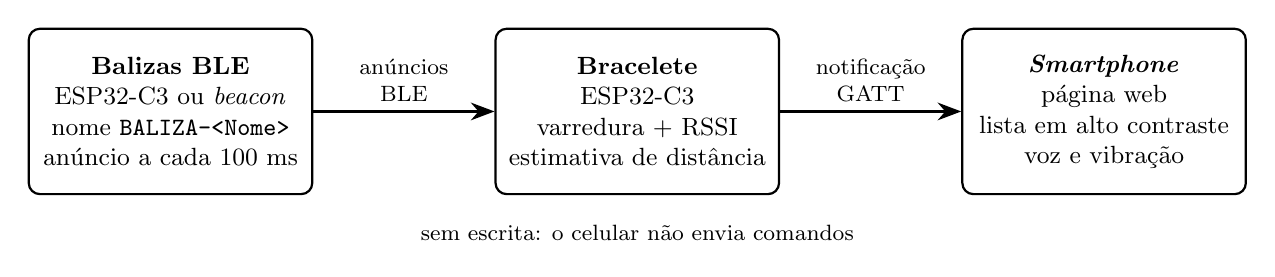
\begin{tikzpicture}[
    bloco/.style={draw, rounded corners, thick, align=center, minimum width=3.6cm, minimum height=2.1cm, font=\small},
    seta/.style={-{Stealth[length=3mm]}, thick},
    rot/.style={font=\footnotesize, align=center}
]
\node[bloco] (baliza) {\textbf{Balizas BLE}\\ESP32-C3 ou \textit{beacon}\\nome \texttt{BALIZA-<Nome>}\\anúncio a cada 100~ms};
\node[bloco, right=2.3cm of baliza] (bracelete) {\textbf{Bracelete}\\ESP32-C3\\varredura + RSSI\\estimativa de distância};
\node[bloco, right=2.3cm of bracelete] (celular) {\textbf{\textit{Smartphone}}\\página web\\lista em alto contraste\\voz e vibração};
\draw[seta] (baliza) -- node[rot, above] {anúncios\\BLE} (bracelete);
\draw[seta] (bracelete) -- node[rot, above] {notificação\\GATT} (celular);
\node[rot, below=0.25cm of bracelete] {sem escrita: o celular não envia comandos};
\end{tikzpicture}
\fonte{Elaborado pelos autores (2026).}
\end{figure}

\section{Etapa 1 -- Concepção física e mudança de escopo}
\label{sec:etapa1}

A primeira versão do projeto seguia a proposta: um sensor ultrassônico HC-SR04 mediria a distância até obstáculos e o motor vibraria com intensidade proporcional. Um primeiro firmware com essa lógica chegou a ser escrito para o ESP32. No detalhamento do projeto, porém, a equipe decidiu retirar o sensor, com dois objetivos: simplificar o hardware do bracelete e concentrar a solução na comunicação sem fio que o ESP32 já oferece. A Figura~\ref{fig:esquema} mostra a concepção física elaborada nessa fase, com microcontrolador, bateria LiPo de 3,7~V, botão liga/desliga e um motor de vibração tipo moeda. O uso desse motor ainda está em avaliação pela equipe, e nesta etapa o retorno ao usuário é dado pelo celular.

\begin{figure}[htb]
\centering
\caption{Esquema técnico da concepção física do bracelete}
\label{fig:esquema}
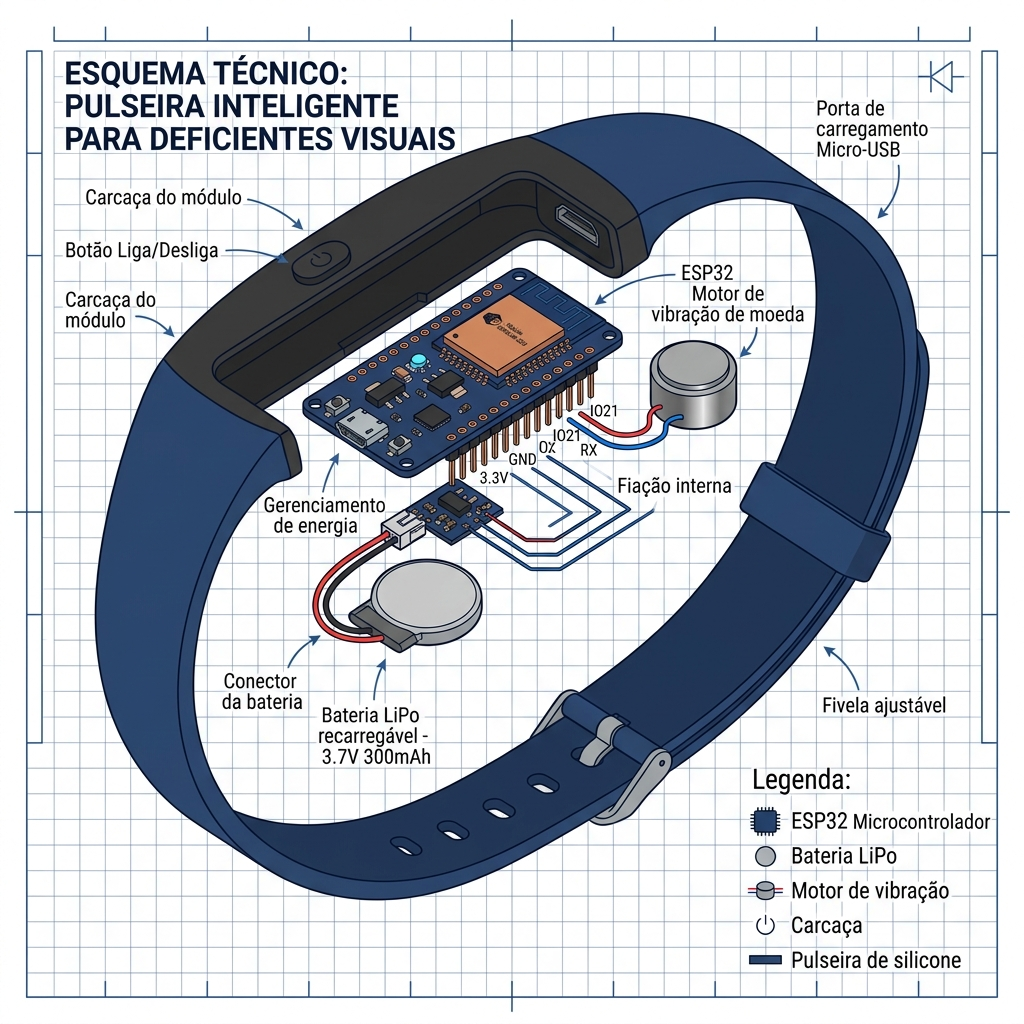
\includegraphics[width=0.62\textwidth]{figuras/esquema_tecnico.jpg}
\fonte{Elaborado pelos autores (2026).}
\end{figure}

Com essa configuração, era preciso outra forma de perceber o ambiente. A alternativa escolhida foi aproveitar o rádio Bluetooth que o ESP32 já possui: pontos de referência do ambiente recebem balizas BLE, e o bracelete estima a proximidade de cada uma pelo sinal. A abordagem não exige componentes extras no bracelete. Em contrapartida, só funciona em ambientes onde as balizas foram instaladas.

\section{Etapa 2 -- Comunicação BLE do bracelete para o celular}
\label{sec:etapa2}

Um requisito definido pela equipe foi que a comunicação ocorresse apenas no sentido bracelete $\rightarrow$ celular. Para isso, o ESP32 foi configurado como servidor GATT com um serviço próprio, identificado por UUID, contendo uma única característica com as propriedades de leitura e notificação e sem escrita. Quando o celular se inscreve nas notificações, o bracelete passa a enviar os dados a cada 500~ms. A comunicação foi validada primeiro com o aplicativo nRF Connect, que exibiu o dispositivo \texttt{Bracelete-ESP32} e os valores recebidos por notificação.

\section{Etapa 3 -- Interface web no celular}
\label{sec:etapa3}

Para dispensar a instalação de aplicativo, a interface foi feita como uma página web estática que usa Web Bluetooth para se conectar ao bracelete. A página foi publicada no GitHub Pages, que fornece o HTTPS exigido pela API. O desenho da interface seguiu três princípios voltados à baixa visão:
\begin{itemize}
    \item fundo preto com texto grande e cores de alto contraste;
    \item cores diferentes por faixa de proximidade;
    \item anúncio por voz das mudanças.
\end{itemize}
Um botão ``O que tem por perto?'' lê em sequência todos os pontos detectados, do mais próximo para o mais distante. A Figura~\ref{fig:interface} mostra a versão atual da interface.

\begin{figure}[htb]
\centering
\caption{Interface web exibindo três pontos no modo demonstração}
\label{fig:interface}
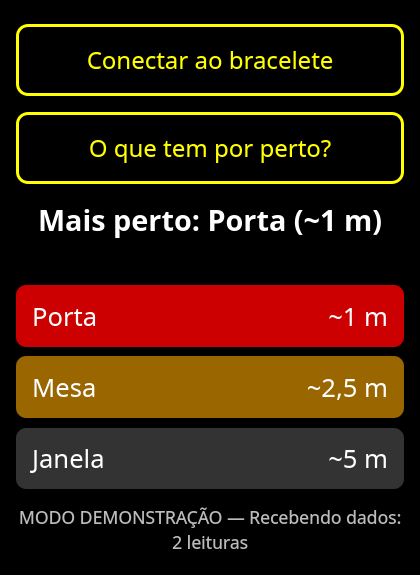
\includegraphics[width=0.36\textwidth]{figuras/interface_web_demo.png}
\fonte{Elaborado pelos autores (2026). Captura em navegador de computador, com mensagem no formato enviado pelo bracelete no modo demonstração.}
\end{figure}

Uma decisão de segurança foi tomada durante os testes. A primeira versão exibia ``Caminho livre'' quando o sensor não retornava leitura, o que poderia induzir o usuário a erro. A interface passou a diferenciar a ausência de leitura, informando ``Nenhuma baliza por perto'', e nunca anuncia caminho livre.

\section{Etapa 4 -- Migração para o ESP32-C3}
\label{sec:etapa4}

O firmware foi escrito inicialmente para o ESP32 convencional. A placa disponível, porém, era um ESP32-C3, identificado pela ferramenta \texttt{esptool}, o que exigiu três ajustes:
\begin{itemize}
    \item \textbf{pinos:} os GPIO 18 e 19, usados antes, correspondem ao USB nativo do C3, e os GPIO 2, 8 e 9 são pinos de inicialização. A saída reservada ao motor foi movida para o GPIO~5;
    \item \textbf{saída serial:} foi necessário habilitar a opção \textit{USB CDC On Boot} para que a saída serial fosse enviada pela USB;
    \item \textbf{PWM:} as funções de PWM foram atualizadas para a API da versão 3 do núcleo Arduino-ESP32.
\end{itemize}
Para simplificar a gravação sem a IDE do Arduino, foi criado um \textit{script} que compila, grava e abre o monitor serial com o \texttt{arduino-cli}.

\section{Etapa 5 -- Modo demonstração}
\label{sec:etapa5}

Para permitir apresentações sem depender de balizas instaladas, foi criado um modo demonstração, ligado e desligado pelo botão BOOT da placa. Nesse modo, o bracelete simula três balizas (``Porta'', ``Mesa'' e ``Janela'') com distâncias que variam ciclicamente, e a interface indica claramente ``MODO DEMONSTRAÇÃO'' para não ser confundida com uma leitura real. O modo sempre inicia desligado.

\section{Etapa 6 -- Detecção de múltiplas balizas}
\label{sec:etapa6}

Nesta etapa foi implementada a detecção por balizas, com dois programas:
\begin{itemize}
    \item \textbf{Firmware da baliza:} o ESP32-C3 anuncia o nome \texttt{BALIZA-<Nome>} a cada 100~ms, com potência de transmissão fixa, para que a relação entre sinal e distância seja estável;
    \item \textbf{Firmware do bracelete:} faz varredura contínua ativa, com janela de 50~ms a cada 100~ms, deixando tempo de rádio para a conexão com o celular. Ele mantém uma tabela de até oito balizas com o RSSI suavizado pela Equação~\ref{eq:ema}, usando $\alpha = 0{,}15$, e descarta a baliza que fica mais de 6~s sem ser ouvida.
\end{itemize}

A distância é calculada pela Equação~\ref{eq:distancia}, com valores iniciais $A = -59$~dBm e $n = 2{,}5$, e classificada em três faixas (até 1~m, até 2~m e até 4~m). Para evitar que os alertas fiquem alternando na fronteira de uma faixa, foi aplicada uma histerese: para voltar a uma faixa mais distante, a estimativa precisa ultrapassar o limite em 25\%.

A mensagem enviada ao celular segue o formato \texttt{<demo>|Nome:cm;Nome:cm;...}, com as balizas ordenadas da mais próxima para a mais distante e limitada ao tamanho máximo do pacote negociado na conexão (MTU). Na interface, um ponto novo só é anunciado após duas leituras seguidas. O mesmo ponto não é anunciado de novo em menos de 4~s, e as falas entram em fila em vez de interromper a anterior. Apenas a aproximação a menos de 1~m interrompe a fala em andamento, por ser o alerta mais urgente. O Apêndice~\ref{ap:codigo} traz os principais trechos do código.

\section{Etapa 7 -- Procedimentos de teste}
\label{sec:etapa7}

Os testes foram feitos de forma incremental, após cada etapa:
\begin{enumerate}
    \item \textbf{compilação:} todos os programas foram compilados e o uso de memória foi registrado;
    \item \textbf{comunicação:} o bracelete foi conectado ao nRF Connect e depois à interface web, verificando a chegada das notificações;
    \item \textbf{balizas simuladas:} o notebook foi configurado com o BlueZ para anunciar uma e depois duas balizas, e a saída serial do bracelete foi registrada por cerca de 45~s com um \textit{script} em Python, que contou as leituras e as entradas e saídas de balizas;
    \item \textbf{baliza real:} a segunda placa ESP32-C3 foi gravada como baliza ``Porta'' e posicionada a diferentes distâncias do bracelete, observando a distância indicada na interface.
\end{enumerate}

\chapter{RESULTADOS PARCIAIS E DISCUSSÃO}
\label{cap:resultados}

Este capítulo apresenta os resultados obtidos até o momento. Os testes realizados são funcionais e exploratórios, feitos pela equipe em ambiente doméstico e de laboratório. Ainda não houve testes com pessoas do público-alvo, previstos para a etapa final.

\section{Compilação e uso de memória}
\label{sec:res-memoria}

A Tabela~\ref{tab:memoria} mostra o espaço de memória de programa ocupado por cada versão do firmware. Todas as versões compilaram sem erros e ocupam menos da metade da área disponível no ESP32-C3, o que deixa margem para as próximas funcionalidades.

\begin{table}[htb]
\centering
\caption{Memória de programa ocupada por versão do firmware}
\label{tab:memoria}
\small
\begin{tabular}{lcrr}
\toprule
\textbf{Versão} & \textbf{Placa} & \textbf{Bytes} & \textbf{Uso} \\
\midrule
Protótipo inicial (sensor + BLE) & ESP32 & 1.104.594 & 84\% \\
Bracelete com sensor + BLE & ESP32-C3 & 639.133 & 48\% \\
Bracelete com balizas (atual) & ESP32-C3 & 651.955 & 49\% \\
Baliza & ESP32-C3 & 617.933 & 47\% \\
\bottomrule
\end{tabular}
\normalsize
\fonte{Saída do compilador \texttt{arduino-cli}. Área máxima de programa: 1.310.720 bytes.}
\end{table}

\section{Comunicação bracelete $\rightarrow$ celular}
\label{sec:res-comunicacao}

O bracelete foi encontrado pelo aplicativo nRF Connect com o nome \texttt{Bracelete-ESP32}, e as notificações chegaram continuamente após a inscrição. Em seguida, a interface web publicada no GitHub Pages conectou-se ao bracelete pelo Chrome no Android, anunciou ``Bracelete conectado'' por voz e passou a exibir os dados recebidos. Durante o teste, a primeira versão da interface aparentava estar parada, porque só falava quando o valor mudava. Foi então adicionado um contador de leituras recebidas, que mostra ao usuário que a conexão está ativa. O modo demonstração foi verificado pela saída serial: após o acionamento do botão, as 898 linhas registradas em 90~s indicavam o modo ativo, com a distância simulada variando como esperado.

\section{Detecção de balizas simuladas}
\label{sec:res-simuladas}

No primeiro teste com balizas, o notebook anunciou uma baliza chamada ``Mesa'', que o bracelete detectou em 94 leituras consecutivas, com distância estimada de cerca de 1,36~m. Em seguida, o notebook anunciou duas balizas ao mesmo tempo (``Porta'' e ``Mesa''). A Tabela~\ref{tab:duas-balizas} resume os registros coletados após os primeiros 8~s, descartados para estabilização.

\begin{table}[htb]
\centering
\caption{Detecção simultânea de duas balizas simuladas pelo notebook}
\label{tab:duas-balizas}
\small
\begin{tabular}{lcccc}
\toprule
\textbf{Baliza} & \textbf{Leituras} & \textbf{Mínimo (cm)} & \textbf{Mediana (cm)} & \textbf{Máximo (cm)} \\
\midrule
Porta & 182 & 90 & 109 & 124 \\
Mesa & 168 & 123 & 129 & 138 \\
\bottomrule
\end{tabular}
\normalsize
\fonte{Registros da porta serial do bracelete, coletados pelos autores (2026).}
\end{table}

As duas balizas foram detectadas simultaneamente, e as estimativas de cada uma variaram pouco, com amplitude de no máximo 34~cm. No entanto, as duas vinham do mesmo adaptador Bluetooth, portanto estavam exatamente à mesma distância física, e ainda assim as medianas diferiram em 20~cm. Isso mostra que, mesmo em condição controlada, a estimativa depende de fatores além da distância. Também foram registradas 10 entradas e saídas de balizas na lista durante o teste. Parte delas pode ser atribuída ao notebook, que alterna entre os dois anúncios, e parte à própria varredura do bracelete, que escuta o rádio em apenas metade do tempo para manter a conexão com o celular. Esse comportamento motivou os ajustes da Etapa~6: tempo de 6~s para descartar uma baliza, confirmação em duas leituras e fila de falas.

\section{Detecção com baliza real e estimativa de distância}
\label{sec:res-real}

Com a segunda placa ESP32-C3 gravada como baliza ``Porta'', o bracelete detectou a baliza e a interface passou a anunciá-la. A distância exibida, porém, ficou longe da real. A Tabela~\ref{tab:baliza-real} reúne as observações feitas pela interface. A coluna de RSSI equivalente foi calculada invertendo a Equação~\ref{eq:distancia} com $A=-59$~dBm e $n=2{,}5$.

\begin{table}[htb]
\centering
\caption{Distância indicada pela interface com a baliza real}
\label{tab:baliza-real}
\small
\begin{tabular}{p{3.3cm}p{3.2cm}cc}
\toprule
\textbf{Potência da baliza} & \textbf{Distância real} & \textbf{Indicada} & \textbf{RSSI equivalente} \\
\midrule
0 dBm & placas encostadas & $\approx$ 3~m & $\approx -71$~dBm \\
+9 dBm & $\approx$ 30~cm & $\approx$ 1,5~m & $\approx -63$~dBm \\
+9 dBm & 1~m & $\approx$ 20~m & $\approx -92$~dBm \\
\bottomrule
\end{tabular}
\normalsize
\fonte{Observações dos autores na interface web (2026). Valores arredondados pela interface a cada 0,5~m.}
\end{table}

O aumento da potência de transmissão da baliza de 0 para +9~dBm melhorou a detecção a curta distância, mas não resolveu a estimativa. Entre cerca de 30~cm e 1~m, o modelo prevê uma queda de aproximadamente 13~dB no RSSI ($25 \cdot \log_{10}(1/0{,}3)$). A queda equivalente observada foi de cerca de 28~dB, mais que o dobro. Esse resultado é coerente com o que \citeonline{faragher2015} relatam sobre a variabilidade do RSSI, agravada aqui por dois fatores:
\begin{itemize}
    \item a antena impressa das placas SuperMini é pequena, e a orientação relativa das placas altera bastante o sinal recebido;
    \item o valor de $A=-59$~dBm foi adotado como estimativa inicial, sem medição com o par de placas usado.
\end{itemize}
A calibração com leituras brutas de RSSI em posições conhecidas ficou pendente, porque exige o bracelete conectado ao computador por cabo de dados durante a medição.

A conclusão parcial é que, com o hardware atual, \textbf{informar a distância em metros não é confiável} e pode confundir o usuário. Por outro lado, o sinal permite distinguir situações bem diferentes, como a baliza encostada, na mesma área ou distante. Por isso, a próxima versão substituirá os metros por zonas de proximidade (``muito perto'', ``perto'' e ``na sala''), com limites de RSSI definidos por medição.

\section{Dificuldades encontradas e soluções}
\label{sec:res-dificuldades}

O Quadro~\ref{qua:dificuldades} resume os principais problemas técnicos encontrados até aqui e como foram resolvidos.

\begin{quadro}[htb]
\caption{Dificuldades encontradas e soluções adotadas}
\label{qua:dificuldades}
\small
\begin{tabular}{|p{6.4cm}|p{7.6cm}|}
\hline
\textbf{Dificuldade} & \textbf{Solução} \\
\hline
Placa disponível era ESP32-C3, com GPIO 18/19 ligados ao USB & Remapeamento dos pinos (saída do motor no GPIO~5) e compilação para o C3 \\
\hline
Saída serial não aparecia pela USB & Opção \textit{USB CDC On Boot} habilitada na compilação \\
\hline
Funções de PWM removidas na versão 3 do núcleo & Uso da nova API \texttt{ledcAttach}/\texttt{ledcWrite} \\
\hline
Publicação da página no GitHub Pages falhava & Desativação do processamento Jekyll com o arquivo \texttt{.nojekyll} \\
\hline
Interface anunciava ``Caminho livre'' sem leitura & Estado próprio para ausência de dados, sem anúncio de caminho livre \\
\hline
Botão do modo demonstração perdia toques rápidos & Leitura do botão por interrupção em vez de consulta no laço principal \\
\hline
Baliza aparecia e sumia; falas interrompidas & Suavização do RSSI, 6~s para descartar, histerese de 25\%, confirmação em duas leituras e fila de falas \\
\hline
Placa da baliza reiniciava em modo de gravação & Reconexão do cabo USB sem acionar o botão BOOT (pino de inicialização GPIO~9) \\
\hline
Lista de balizas maior que o pacote BLE padrão & Aumento do MTU para 247 bytes e corte da lista no limite negociado \\
\hline
Distância em metros instável com placas SuperMini & Aumento da potência da baliza para +9~dBm; troca por zonas de proximidade em andamento \\
\hline
\end{tabular}
\normalsize
\fonte{Elaborado pelos autores (2026).}
\end{quadro}

\chapter{CONSIDERAÇÕES PARCIAIS E PRÓXIMAS ETAPAS}
\label{cap:consideracoes}

\section{Situação das atividades}
\label{sec:situacao}

O Quadro~\ref{qua:situacao} compara as atividades previstas na proposta com o estado atual. A parte de software está praticamente pronta. Faltam a calibração da proximidade, a montagem física do bracelete e as atividades com o público-alvo.

\begin{quadro}[htb]
\caption{Situação das atividades previstas na proposta}
\label{qua:situacao}
\small
\begin{tabular}{|p{5.4cm}|p{2.4cm}|p{6.2cm}|}
\hline
\textbf{Atividade prevista} & \textbf{Situação} & \textbf{Observação} \\
\hline
1. Pesquisa e levantamento de requisitos & Concluída & Ampliada para BLE, RSSI e Web Bluetooth após a mudança de escopo \\
\hline
2. Projeto e montagem do bracelete & Parcial & Projeto definido; montagem de motor, bateria e pulseira pendente \\
\hline
3. Programação do ESP32 e integração & Concluída & Firmware do bracelete e da baliza, interface web e modo demonstração \\
\hline
4. Testes, avaliação e apresentação & Em andamento & Testes funcionais feitos; calibração, testes com usuários e apresentação pendentes \\
\hline
5. Documentação e registro dos resultados & Em andamento & Código versionado e este relatório parcial \\
\hline
\end{tabular}
\normalsize
\fonte{Elaborado pelos autores (2026).}
\end{quadro}

\section{Considerações parciais}
\label{sec:consideracoes-parciais}

Até aqui, a ação mostrou que é possível construir, com duas placas de baixo custo e um celular comum, um sistema em que o bracelete detecta vários pontos de referência e os informa ao usuário por vibração e voz, sem aplicativo instalado e com comunicação em sentido único. A mudança de escopo, de detecção de obstáculos para orientação por balizas, manteve o objetivo geral da proposta, que é ampliar a percepção do ambiente por pessoas com baixa visão. Ela, porém, traz uma limitação que deve ficar clara: o sistema depende de o ambiente ter sido preparado com balizas e não detecta obstáculos não sinalizados.

O principal aprendizado técnico desta etapa foi a distância entre o modelo teórico de propagação e o comportamento real do hardware. A estimativa em metros, que parecia simples na Equação~\ref{eq:distancia}, mostrou-se pouco confiável com antenas pequenas, e a decisão de trocar metros por zonas veio diretamente dos testes. Outro aprendizado foi o cuidado com a informação dada ao usuário. Em uma tecnologia assistiva, anunciar ``caminho livre'' sem ter leitura, ou uma distância errada, pode ser pior do que não anunciar nada.

Para a formação dos extensionistas, a etapa exigiu integrar conteúdos de sistemas embarcados, redes sem fio, programação web e acessibilidade em um mesmo problema, além de lidar com questões práticas que não aparecem em sala de aula, como diferenças entre variantes de microcontrolador, pinos de inicialização e limitações de antena.

\section{Próximas etapas}
\label{sec:proximas}

\begin{enumerate}
    \item \textbf{Calibração:} medir o RSSI bruto com as placas encostadas, a 1~m e a distâncias maiores, em várias orientações, para definir os limites das zonas de proximidade;
    \item \textbf{Zonas de proximidade:} substituir os metros por zonas (``muito perto'', ``perto'' e ``na sala'') no firmware e na interface;
    \item \textbf{Montagem física:} ligar o motor de vibração com transistor de acionamento, alimentar por bateria LiPo e acomodar o conjunto em uma pulseira;
    \item \textbf{Novas balizas:} gravar ou adquirir balizas para, no mínimo, três pontos de uma sala do campus;
    \item \textbf{Validação com o público-alvo:} realizar testes supervisionados com pessoas com baixa visão, colhendo sua percepção sobre a clareza dos alertas;
    \item \textbf{Apresentação e relatório final:} apresentar o protótipo à comunidade acadêmica do IFPR -- Campus Pinhais e registrar os resultados no relatório final.
\end{enumerate}


\postextual

\bibliography{referencias/referencias}

\begin{apendicesenv}
\partapendices
\chapter{Declaração de uso de Inteligência Artificial Generativa (IAG)}
\label{ap:iag}

\noindent
Em conformidade com a Portaria CNPq nº 2.664, de 6 de março de 2026 \cite{cnpq2026portaria}, que determina a declaração do uso de ferramentas de Inteligência Artificial Generativa (IAG) em qualquer fase do trabalho, especificando a ferramenta e a finalidade, apresenta-se a seguir a declaração relativa a este relatório parcial.

\bigskip
\begin{center}
\textbf{\large DECLARAÇÃO DE USO DE INTELIGÊNCIA ARTIFICIAL GENERATIVA}
\end{center}

\bigskip
\noindent
Nós, \textbf{Matheus Vitor Lourenço Schionato} e \textbf{Vairtles Nehisen Mounkassa Liel}, discentes da disciplina de Práticas de Extensão V do curso de Bacharelado em Ciência da Computação do IFPR -- Campus Pinhais, declaramos que fizemos uso de ferramenta de IAG no desenvolvimento desta etapa do trabalho, conforme especificado abaixo:

\bigskip
\begin{center}
\small
\begin{tabular}{|p{4.2cm}|p{9.8cm}|}
\hline
\textbf{Ferramenta utilizada} & Claude Code (Anthropic), assistente de programação baseado em modelo de linguagem, executado no terminal do computador dos autores \\
\hline
\textbf{Fases em que houve uso} &
\begin{itemize}[leftmargin=*, nosep]
  \item[$\blacksquare$] Concepção (apoio na avaliação de alternativas técnicas)
  \item[$\blacksquare$] Redação
  \item[$\blacksquare$] Análise de dados
  \item[$\square$] Submissão
\end{itemize} \\
\hline
\textbf{Finalidade do uso} &
\begin{itemize}[leftmargin=*, nosep]
  \item apoio à escrita do firmware do bracelete e da baliza e da interface web;
  \item automação da compilação, gravação e coleta dos registros seriais;
  \item resumo estatístico dos registros de teste (contagens, mínimos, medianas e máximos);
  \item redação preliminar deste relatório a partir das atividades e dos dados do projeto.
\end{itemize} \\
\hline
\end{tabular}
\end{center}

\bigskip
\noindent
Declaramos, ainda, que:
\begin{enumerate}[label=\alph*)]
  \item os dados de teste apresentados foram obtidos com o hardware real ou com as simulações descritas no texto, e não foram gerados pela ferramenta;
  \item as decisões de projeto, como a configuração do bracelete sem sensor e a adoção de balizas BLE, foram tomadas pelos autores;
  \item todo o conteúdo, inclusive o código e o texto produzidos com apoio da ferramenta, foi revisado por nós, que assumimos integral responsabilidade por ele;
  \item não foram inseridos na ferramenta projetos de terceiros nem dados sigilosos.
\end{enumerate}

\bigskip
\noindent
Pinhais, 29 de setembro de 2026.

\bigskip\bigskip\bigskip
\begin{center}
\begin{tabular}{cc}
\rule{6.5cm}{0.5pt} & \rule{6.5cm}{0.5pt} \\
\textbf{Matheus Vitor Lourenço Schionato} & \textbf{Vairtles Nehisen Mounkassa Liel} \\
Discente extensionista -- IFPR & Discente extensionista -- IFPR
\end{tabular}
\end{center}

\chapter{Principais trechos do firmware do bracelete}
\label{ap:codigo}

\lstset{
  basicstyle=\ttfamily\footnotesize,
  columns=fullflexible,
  keepspaces=true,
  frame=single,
  breaklines=true,
  showstringspaces=false,
  language=C++
}

Os trechos a seguir foram extraídos do firmware do bracelete (\texttt{bracelete\_ble.ino}). O código completo, o firmware da baliza e a interface web estão no repositório do projeto.

\section{Recebimento dos anúncios e suavização do RSSI}

A cada anúncio recebido, o bracelete verifica se o nome começa com \texttt{BALIZA-} e atualiza o RSSI suavizado da baliza correspondente (Equação~\ref{eq:ema}).

\begin{lstlisting}
void onResult(BLEAdvertisedDevice dev) override {
  if (!dev.haveName()) return;
  String full = dev.getName();
  if (!full.startsWith(BEACON_PREFIX)) return;
  String name = full.substring(strlen(BEACON_PREFIX));
  int rssi = dev.getRSSI();
  ...
  if (slot < 0) {                       // baliza nova
    strlcpy(beacons[slot].name, name.c_str(), sizeof(beacons[slot].name));
    beacons[slot].rssi = rssi;
  } else {                              // media movel exponencial
    beacons[slot].rssi += RSSI_ALPHA * (rssi - beacons[slot].rssi);
  }
  beacons[slot].lastSeen = now;
}
\end{lstlisting}

\section{Estimativa de distância e histerese}

\begin{lstlisting}
int rssiToCm(float rssi) {              // Equacao (1), em centimetros
  return 100 * pow(10, (RSSI_1M - rssi) / (10 * PATH_LOSS_N));
}

const int LIMITS[] = {400, 200, 100};   // faixas: 4 m, 2 m e 1 m

int levelWithHysteresis(int cm, int current) {
  int level = 0;
  for (int i = 0; i < 3; i++) if (cm <= LIMITS[i]) level = i + 1;
  if (level < current && cm <= LIMITS[current - 1] * 1.25) return current;
  return level;
}
\end{lstlisting}

\section{Característica sem escrita e envio ao celular}

A característica é criada apenas com leitura e notificação, o que garante o fluxo em sentido único. No laço principal, a lista de balizas é montada da mais próxima para a mais distante e enviada a cada 500~ms.

\begin{lstlisting}
distChar = service->createCharacteristic(
    DIST_CHAR_UUID,
    BLECharacteristic::PROPERTY_READ | BLECharacteristic::PROPERTY_NOTIFY);

// laco principal: "<demo>|Nome:cm;Nome:cm;..."
String payload = String(demoMode ? 1 : 0) + "|";
if (connected && now - lastNotify >= NOTIFY_MS) {
  size_t maxLen = server->getPeerMTU(server->getConnId()) - 3;
  for (int i = 0; i < n; i++) {
    String item = String(i ? ";" : "") + points[i].name + ":" + points[i].cm;
    if (payload.length() + item.length() > maxLen) break;
    payload += item;
  }
  distChar->setValue(payload.c_str());
  distChar->notify();
  lastNotify = now;
}
\end{lstlisting}

\end{apendicesenv}

\end{document}
